\chapter{Use case}\label{ch:usecase}
To illustrate the simplicity of the library we implemented a use case, called \textit{Plateforme DD}. The goal was to visualize the links between the content of the website\footnote{https://sciences.brussels/dd/}. The visualization and functionality is completely different than the one for GuideaMaps and can be seen in figure \ref{fig:plateforme-dd}.\\

\begin{figure}[H]
	\centering
	\frame{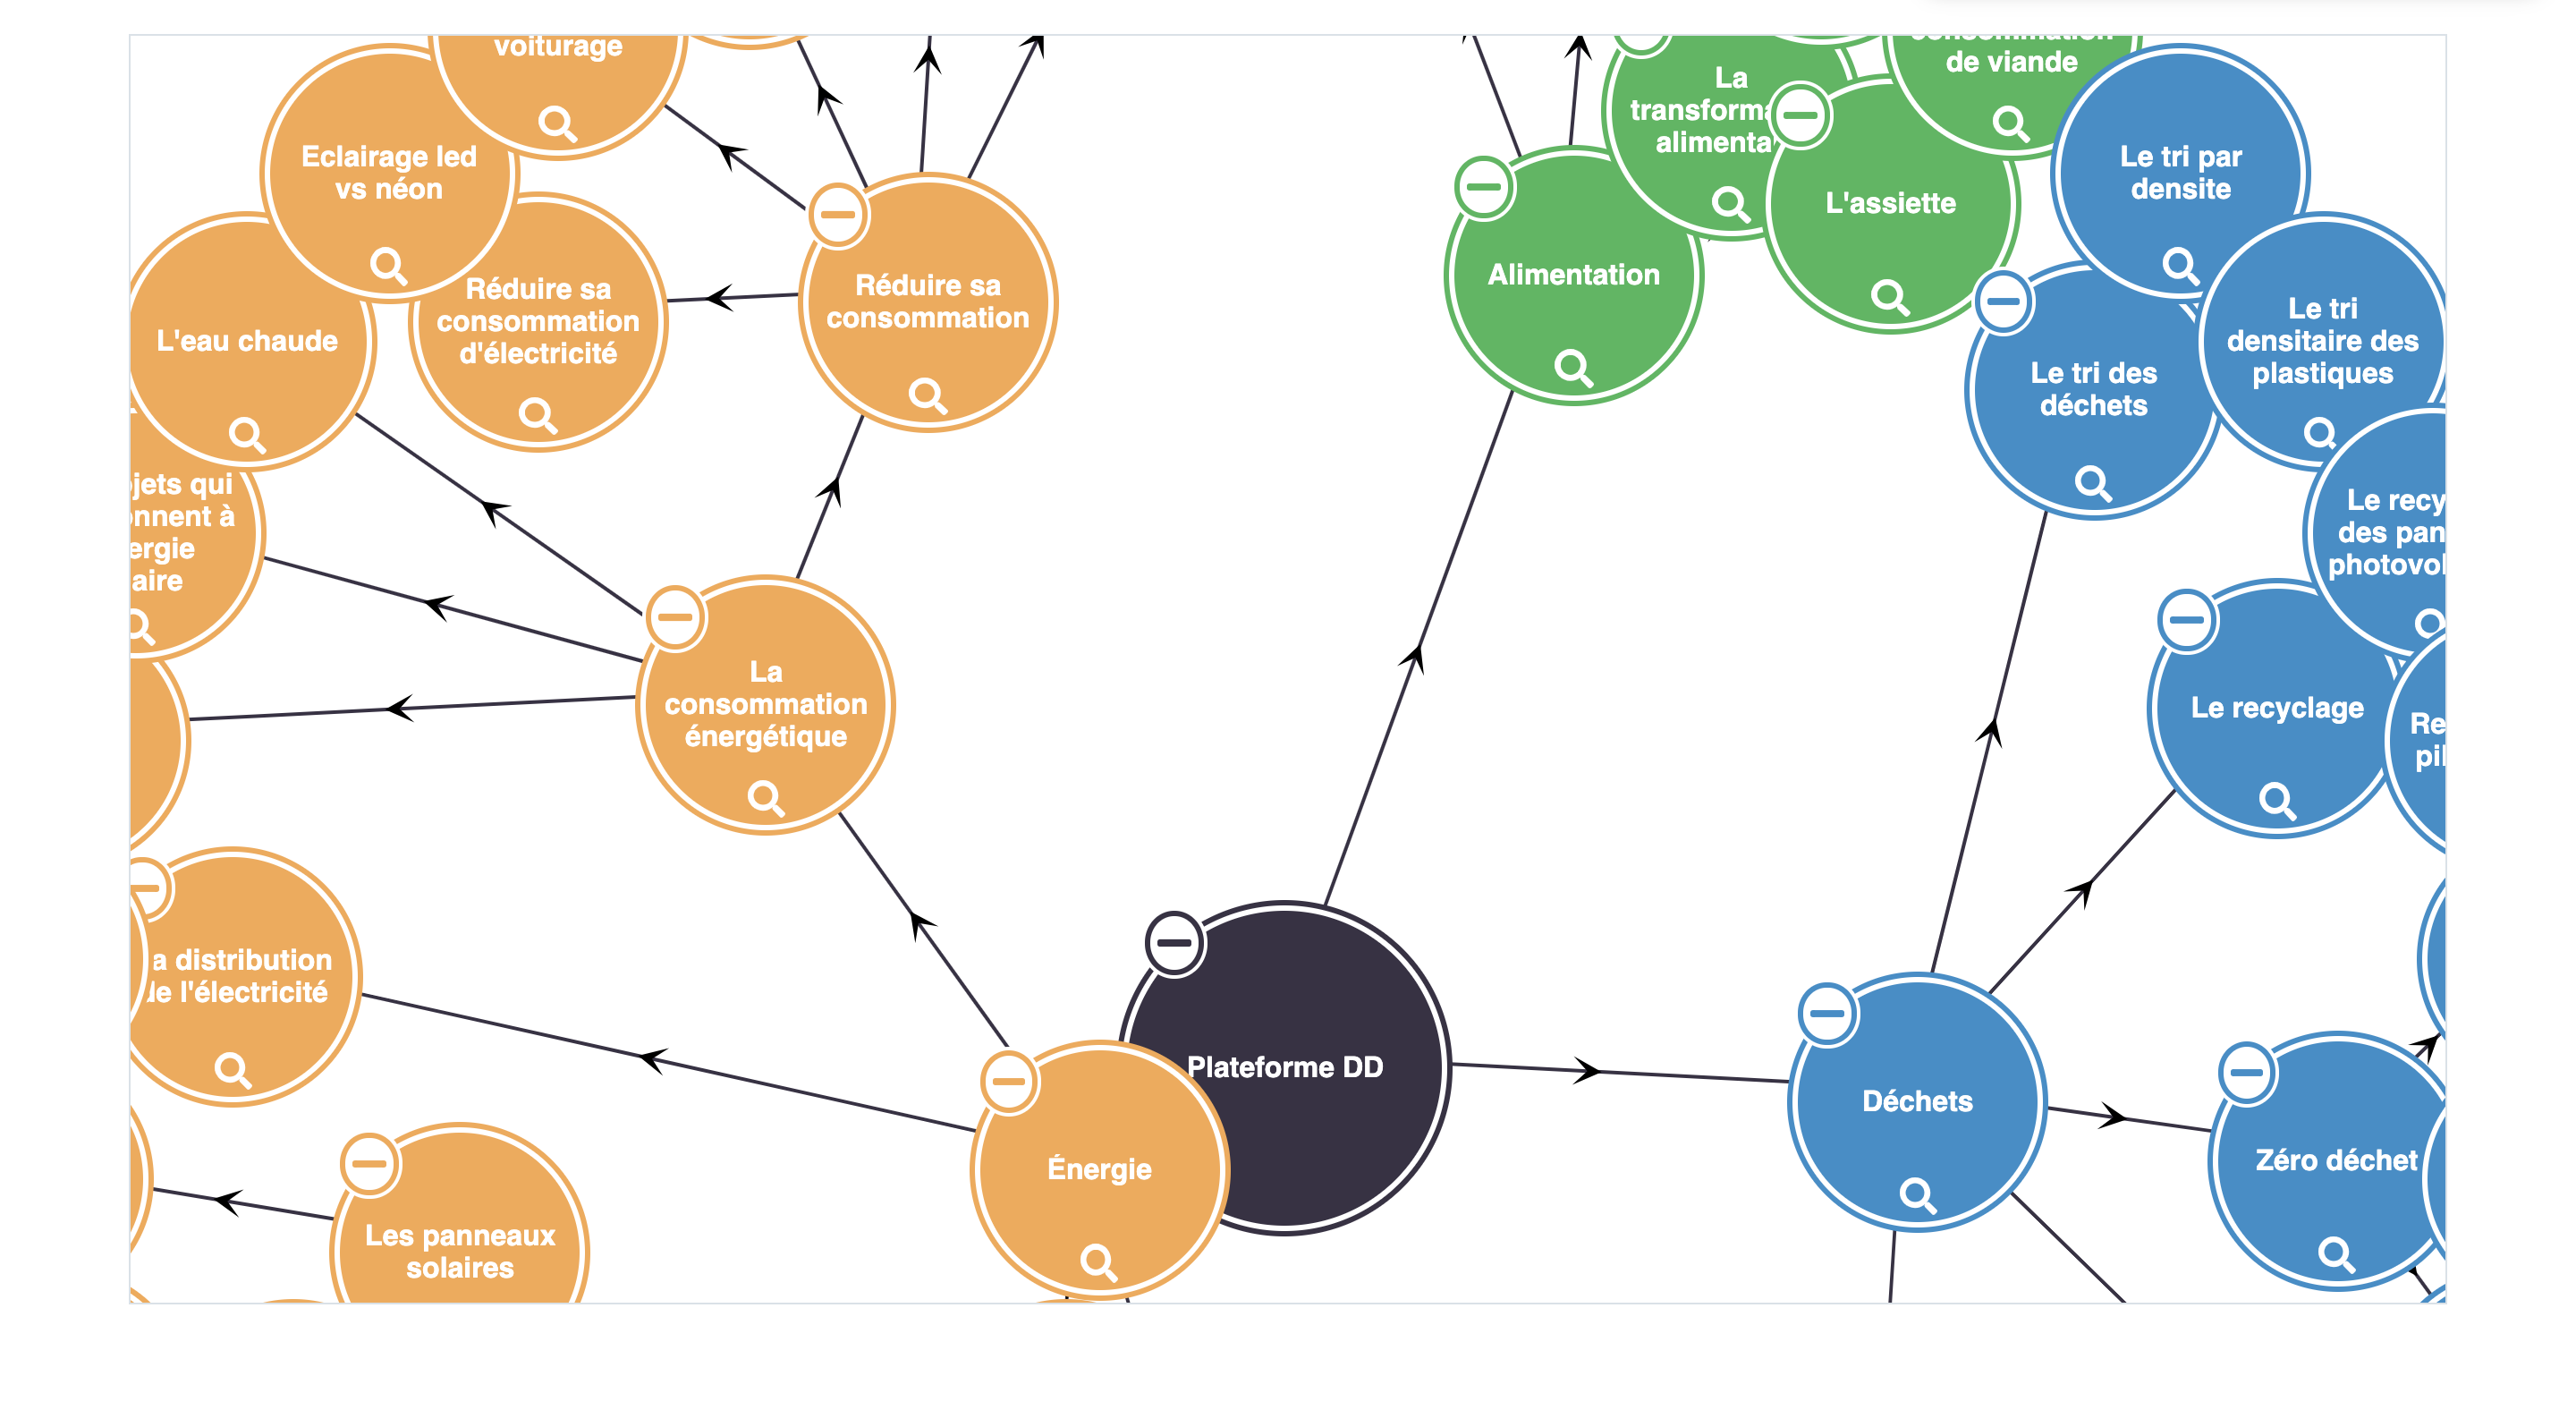
\includegraphics[width=\linewidth]{plateforme-dd.png}}
	\caption{Plateforme DD Layout.}
	\label{fig:plateforme-dd}
\end{figure}

The most obvious difference, which can immediately be seen, is the layout of the nodes. In GuideaMaps (GM), we had rectangular nodes, while in Plateforme DD (PDD) the nodes are circular. To achieve this result, we implemented a special component, called \textit{PDDNode}, and plugged it in the library like we did in Figure \ref{fig:examplecode-library}. In this case \textit{MyCustomNode} is equal to \textit{PDDNode}.\\

As already mentioned in section \ref{sec:structure}, these are not the only customizable props of the library. Figure \ref{fig:differences-gm-vs-pdd} shows the differences in configuration when we compare the visualization of GuideaMaps with the one of Plateforme DD.

\begin{figure}[H]
	\begin{minipage}{0.5\textwidth}
 		 \centering
		 \begin{minted}[linenos, escapeinside=||]{html}
<ZoomableTree
    |\textcolor{mygreen}{NodeComp}|=|\textcolor{red}{\{GMNode\}}|
    |\textcolor{mygreen}{LinkComp}|=|\textcolor{red}{\{GMLink\}}|
    |\textcolor{mygreen}{EditModalComp}|=|\textcolor{red}{\{GMEditModal\}}|
    |\textcolor{mygreen}{onAddNode}|=|\textcolor{red}{\{addGMNode\}}|
    |\textcolor{mygreen}{onDeleteNode}|=|\textcolor{red}{\{deleteGMNode\}}|
/>
		\end{minted}
		\label{lst:default-components}
		\captionof{lstlisting}{GM Configuration.}
	\end{minipage}
 	\begin{minipage}{0.5\textwidth}
  		\centering
  		\begin{minted}[escapeinside=||]{html}
<ZoomableTree
    |\textcolor{mygreen}{NodeComp}|=|\textcolor{red}{\{PDDNode\}}|
    |\textcolor{mygreen}{LinkComp}|=|\textcolor{red}{\{PDDLink\}}|
    |\textcolor{mygreen}{EditModalComp}|=|\textcolor{red}{\{PDDEditModal\}}|
    |\textcolor{mygreen}{onAddNode}|=|\textcolor{red}{\{() -> null\}}|
    |\textcolor{mygreen}{onDeleteNode}|=|\textcolor{red}{\{() -> null\}}|
/>
		\end{minted}
		\label{lst:custom-components}
 	 	\captionof{lstlisting}{PDD Configuration.}
 	\end{minipage}
	\caption{The configuration differences between GuideaMaps and Plateforme DD.}
	\label{fig:differences-gm-vs-pdd}
 	%\captionof{figure}{Two listings showing the difference between the default and custom use of the library.}
\end{figure}